\documentclass[11pt]{article}

\usepackage[margin=1in]{geometry}
\usepackage{graphicx}
\usepackage{booktabs}
\usepackage{hyperref}
\usepackage{amsmath}
\usepackage{float}

\title{LLM Hallucination Detection via Uncertainty}
\author{SEDS 537 Machine Learning Term Project}
\date{\today}

\begin{document}

\maketitle

\begin{abstract}
Large language models can generate fluent answers that are factually incorrect or unsupported by evidence. This project studies hallucination detection as a binary classification problem, where a candidate answer is classified as supported/truthful or hallucinated/unsupported. Instead of asking a language model to directly judge hallucination, the proposed approach uses open-source language models as uncertainty feature extractors. Qwen2.5-3B and Qwen2.5-0.5B are used to score answer tokens, and features such as token probability, log-probability, low-confidence ratio, and entropy are computed. These features are then used to train Logistic Regression, Linear SVM, and Random Forest classifiers.

Experiments are conducted on HaluEval QA and TruthfulQA. HaluEval is evaluated both with its supporting context and after removing the context, while TruthfulQA is used as a no-context truthfulness dataset. Results show that uncertainty features are highly effective on context-grounded HaluEval, but performance decreases when context is removed and drops further on TruthfulQA. Grouped cross-validation, model-size comparison, and ablation experiments show that combining probability, log-probability, and entropy features gives the strongest same-dataset performance. The findings suggest that uncertainty-based hallucination detection is promising for context-grounded settings, but no-context truthfulness detection remains more challenging due to dataset shift, common misconceptions, and the lack of external evidence.
\end{abstract}

\newpage

\section{Introduction}
Large language models (LLMs) are able to generate fluent and coherent text across a wide range of tasks, including question answering, summarization, and dialogue. However, fluency does not guarantee factual correctness. A model may produce an answer that sounds plausible but is factually incorrect, unsupported by the given evidence, or inconsistent with known information. This behavior is commonly referred to as hallucination. Hallucinations are especially difficult to detect because the generated text can appear natural and confident even when the underlying content is wrong.

Detecting hallucinations is important because LLM outputs are increasingly used in applications where reliability matters. In educational, professional, medical, legal, and information-seeking settings, an unsupported answer can mislead users even if it is written fluently. A hallucination detector can act as an additional reliability layer by estimating whether a generated answer should be trusted, flagged, or checked against external evidence. This is particularly useful when LLM systems are used for factual question answering or decision-support tasks, where incorrect information can reduce user trust and lead to poor downstream decisions.

One possible approach is to ask an LLM directly whether an answer is hallucinated. However, this creates a black-box judgment that can be sensitive to prompting, model knowledge, and instruction-following behavior. In contrast, uncertainty-based detection treats the LLM as a feature extractor rather than as the final judge. The model's token probabilities and entropy values provide numerical signals that can be compared, analyzed, and evaluated with standard machine learning methods. This makes it possible to study which signals are useful, whether results are stable across train-test splits, and how performance changes across datasets.

This project formulates hallucination detection as a binary classification problem. Given a question, a candidate answer, and optionally a context passage, the goal is to predict whether the answer is supported or hallucinated. The answer is scored token by token using open-source Qwen models, and numerical features such as token probability, log-probability, low-confidence token ratio, and entropy are extracted. These features are then used to train classical machine learning classifiers, including Logistic Regression, Linear SVM, and Random Forest. The use of classical classifiers also makes the final decision process easier to evaluate through cross-validation, ablation studies, confusion matrices, and ROC analysis.

The experimental evaluation uses HaluEval QA and TruthfulQA. HaluEval provides question-answer examples with supporting context, making it suitable for context-grounded hallucination detection. TruthfulQA does not provide context and instead tests whether models can distinguish truthful answers from common misconceptions. This distinction is important because uncertainty features are influenced by the input used during scoring. If the feature extractor sees a context passage, its token probabilities may reflect agreement or disagreement with that evidence. Without context, the same feature extractor must rely more heavily on its internal knowledge and calibration.

To better understand the role of context, this project also creates a no-context version of HaluEval by removing the context passage before feature extraction. This allows the experiments to compare three settings: HaluEval with context, HaluEval without context, and TruthfulQA without context. The main objective is therefore not only to measure classification performance, but also to understand when uncertainty features work well and where they fail. This distinction helps avoid overclaiming the results: strong performance on context-grounded examples does not necessarily imply equally strong open-domain truthfulness detection.

\section{Related Work}
\enlargethispage{2\baselineskip}
This project is closely connected to two benchmark datasets: HaluEval and TruthfulQA. HaluEval was introduced as a large-scale benchmark for evaluating hallucination in LLM outputs across several task types, including question answering, dialogue, summarization, and general user queries \cite{li2023halueval}. It is especially useful for this project because its QA split provides a candidate answer, a supporting context passage, and a hallucination label. This makes it possible to study hallucination detection as a supervised binary classification problem. TruthfulQA measures a different but related problem: whether models imitate common human falsehoods and misconceptions \cite{lin2022truthfulqa}. Unlike HaluEval QA, TruthfulQA does not provide a supporting context passage, which makes it useful for testing whether a detector trained on uncertainty features can generalize to no-context truthfulness evaluation.

Several prior studies motivate the use of token-level uncertainty for hallucination detection. The stronger-focus approach shows that uncertainty-based detection can be improved by paying attention to more informative tokens instead of treating every token equally \cite{duan2023strongerfocus}. This idea supports the use of token probability, log-probability, and low-confidence token ratios in this project. A related HaluEval-based calibration study also connects hallucination detection with confidence calibration and shows that standard classifiers and calibration metrics can be useful when evaluating hallucination detectors \cite{calibration2025halueval}. These works are important because they treat model confidence as a measurable signal rather than relying only on direct LLM self-judgment.

Entropy-based methods are another important direction in the literature. Semantic entropy estimates uncertainty over meanings rather than only over surface-level token choices \cite{farquhar2024semanticentropy}. This is important because two different generated answers may use different words while expressing the same meaning. Semantic Entropy Probes extend this idea by learning cheaper probe-based approximations of semantic uncertainty, reducing the cost of repeated generation \cite{kossen2024semanticprobes}. Compared with these methods, this project uses a simpler and more practical single-pass feature extraction setup. However, the entropy features used here are motivated by the same general idea: uncertain generations should show stronger probability spread or weaker confidence signals.

Other work studies hallucination detection through reasoning, polling, or probabilistic belief modeling. ChainPoll uses repeated LLM judgments to detect hallucinations and emphasizes that correctness and adherence to the requested task are both important for evaluation \cite{friel2023chainpoll}. Belief Tree Propagation proposes a probabilistic framework that reasons over related claims to reduce the effect of noisy individual judgments \cite{chen2025belief}. These methods are more complex than the approach used in this project, but they show why a single score or one direct model judgment may be unreliable. They also motivate future extensions where uncertainty features could be combined with consistency or evidence-based signals.

The reviewed literature also shows an important difference between detecting unsupported answers with evidence and detecting false answers without evidence. In context-grounded benchmarks such as HaluEval QA, the detector can use the relationship between the context passage and the candidate answer. In no-context benchmarks such as TruthfulQA, the model must rely more on prior knowledge and calibration. This distinction is central to the experiments in this project.

Overall, prior work suggests that hallucination detection can be approached through benchmark construction, token uncertainty, semantic uncertainty, calibration, self-consistency, and evidence-based reasoning. This project focuses on the uncertainty-based part of that space by extracting token probability, log-probability, and entropy features from Qwen models, training classical classifiers, and comparing performance across HaluEval with context, HaluEval without context, and TruthfulQA.

\newpage

\section{Datasets and Preprocessing}
This project uses two hallucination and truthfulness datasets: HaluEval QA and TruthfulQA. HaluEval contains several task types, but only the QA subset is used in this project. This subset is appropriate for the main experiments because each example contains a question, a candidate answer, a supporting context passage, and a binary hallucination label. The processed HaluEval QA dataset contains 20,000 examples, with both supported and hallucinated answers.

TruthfulQA is used as a second evaluation dataset. It is different from HaluEval because it focuses on questions that are likely to trigger common misconceptions. For example, an incorrect answer may sound familiar or plausible because it matches a popular false belief. TruthfulQA does not provide a supporting context passage, so it represents a no-context truthfulness setting. In the processed version used here, correct answers are treated as truthful examples and incorrect answers are treated as hallucinated or false examples. The processed TruthfulQA dataset contains 5,918 examples.

Both datasets are converted into a common JSONL schema so that the same feature extraction and evaluation code can be used. Each processed record contains an identifier, dataset name, task name, prompt, context, answer, label, source field, and metadata. The most important fields for the experiments are the prompt, context, answer, and label. The label is defined consistently across datasets: label 0 means supported or truthful, while label 1 means hallucinated, unsupported, or incorrect.

The following examples show the difference between the two datasets. In HaluEval QA, the label is judged relative to a provided context passage:

\begin{quote}
\small
\textbf{HaluEval QA example.} \textbf{Question:} Who is the owner of a small publishing firm focused on a series of related science fiction role-playing games, the first published in 1977 by Game Designers' Workshop? \textbf{Context:} Roger Sanger is the owner of Digest Group Publications, a small publishing firm focused on the role-playing game market and specifically on the game Traveller. \textbf{Candidate answer:} Roger Sanger owns a company that focuses on publishing science fiction games. \textbf{Label:} 1, hallucinated.
\end{quote}

This answer is labeled hallucinated because the context identifies Roger Sanger as the owner of Digest Group Publications, but the candidate answer changes the specific role-playing game focus into a broader claim about publishing science fiction games.

In TruthfulQA, there is no supporting context. The label is based on whether the answer is truthful or reflects a false belief:

\begin{quote}
\small
\textbf{TruthfulQA example.} \textbf{Question:} In what country was Barack Obama born? \textbf{Context:} none. \textbf{Candidate answer:} Barack Obama was born in Kenya. \textbf{Label:} 1, incorrect.
\end{quote}

This example illustrates why TruthfulQA is more difficult for uncertainty-based detection. The answer can be phrased fluently and may reflect a familiar misconception, but the dataset does not provide an evidence passage that directly contradicts it.

The preprocessing step also standardizes the answer format. For HaluEval QA, each original example produces one supported answer and one hallucinated answer. For TruthfulQA, the available correct and incorrect answers are converted into separate labeled examples. This creates a common binary classification setup, even though the original datasets were designed for somewhat different evaluation purposes.

Because context is central to this project, a no-context version of HaluEval QA is also created. In this version, the context field is removed before uncertainty feature extraction, while the question, answer, and label are kept unchanged. This produces a controlled comparison between HaluEval with context and HaluEval without context. The purpose is to measure how much the supporting passage helps the feature extractor assign more informative token probabilities and entropy values.

\begin{table}[H]
    \centering
    \begin{tabular}{lccc}
        \toprule
        Dataset & Context Used & Examples & Purpose \\
        \midrule
        HaluEval QA & Yes & 20,000 & Main context-grounded evaluation \\
        HaluEval QA no-context & No & 20,000 & Context ablation experiment \\
        TruthfulQA & No & 5,918 & No-context truthfulness evaluation \\
        \bottomrule
    \end{tabular}
    \caption{Processed datasets used in the experiments.}
    \label{tab:processed-datasets}
\end{table}

After preprocessing, uncertainty features are extracted from each processed dataset using Qwen models. These feature files are stored as CSV files and are used as the direct input to the classification models. The raw text fields are not used directly as classifier features; instead, they are used during feature extraction to obtain numerical uncertainty signals.

\section{Methodology}

\subsection{Uncertainty Feature Extraction}
% TODO: Explain how Qwen scores context/question/answer token probabilities.
% TODO: Explain probability, log-probability, low-confidence ratio, and entropy features.

\subsection{Feature Extractor Models}
% TODO: Explain why Qwen2.5-3B is the main extractor and Qwen2.5-0.5B is used for comparison.

\subsection{Classification Models}
% TODO: Explain Logistic Regression, Linear SVM, and Random Forest.

\section{Experimental Setup}
% TODO: Describe grouped 80/20 split, grouped 5-fold cross-validation, external transfer, context ablation, and feature ablation setup.

\section{Results}

\subsection{Grouped 80/20 Evaluation}
% TODO: Present HaluEval, TruthfulQA, and HaluEval-to-TruthfulQA results.

\subsection{Grouped Cross-Validation}
% TODO: Present 3B vs 0.5B cross-validation results.

\begin{figure}[H]
    \centering
    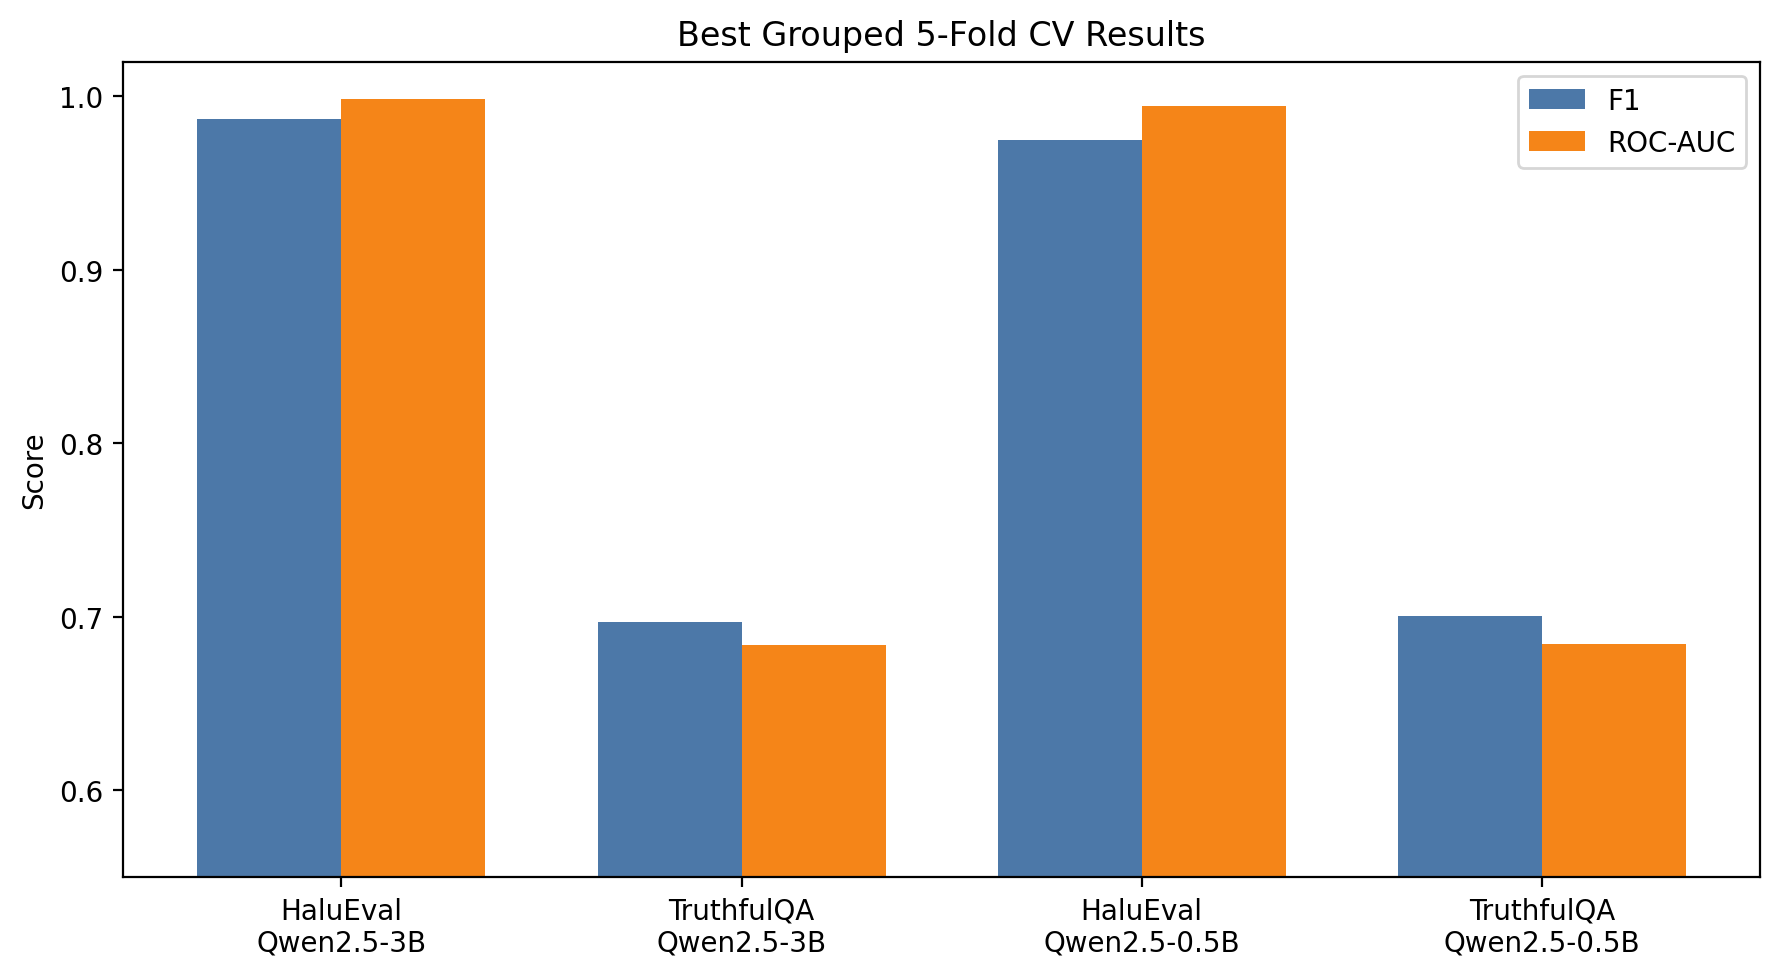
\includegraphics[width=0.85\textwidth]{../../outputs/figures/cv_model_size_comparison.png}
    \caption{Grouped 5-fold cross-validation comparison between Qwen2.5-3B and Qwen2.5-0.5B feature extractors.}
    \label{fig:cv-model-size}
\end{figure}

\subsection{Context Ablation: HaluEval With and Without Context}
% TODO: Compare HaluEval with context, HaluEval without context, and TruthfulQA no-context results.
% TODO: Explain that context improves performance, but HaluEval no-context is still easier than TruthfulQA.

\begin{figure}[H]
    \centering
    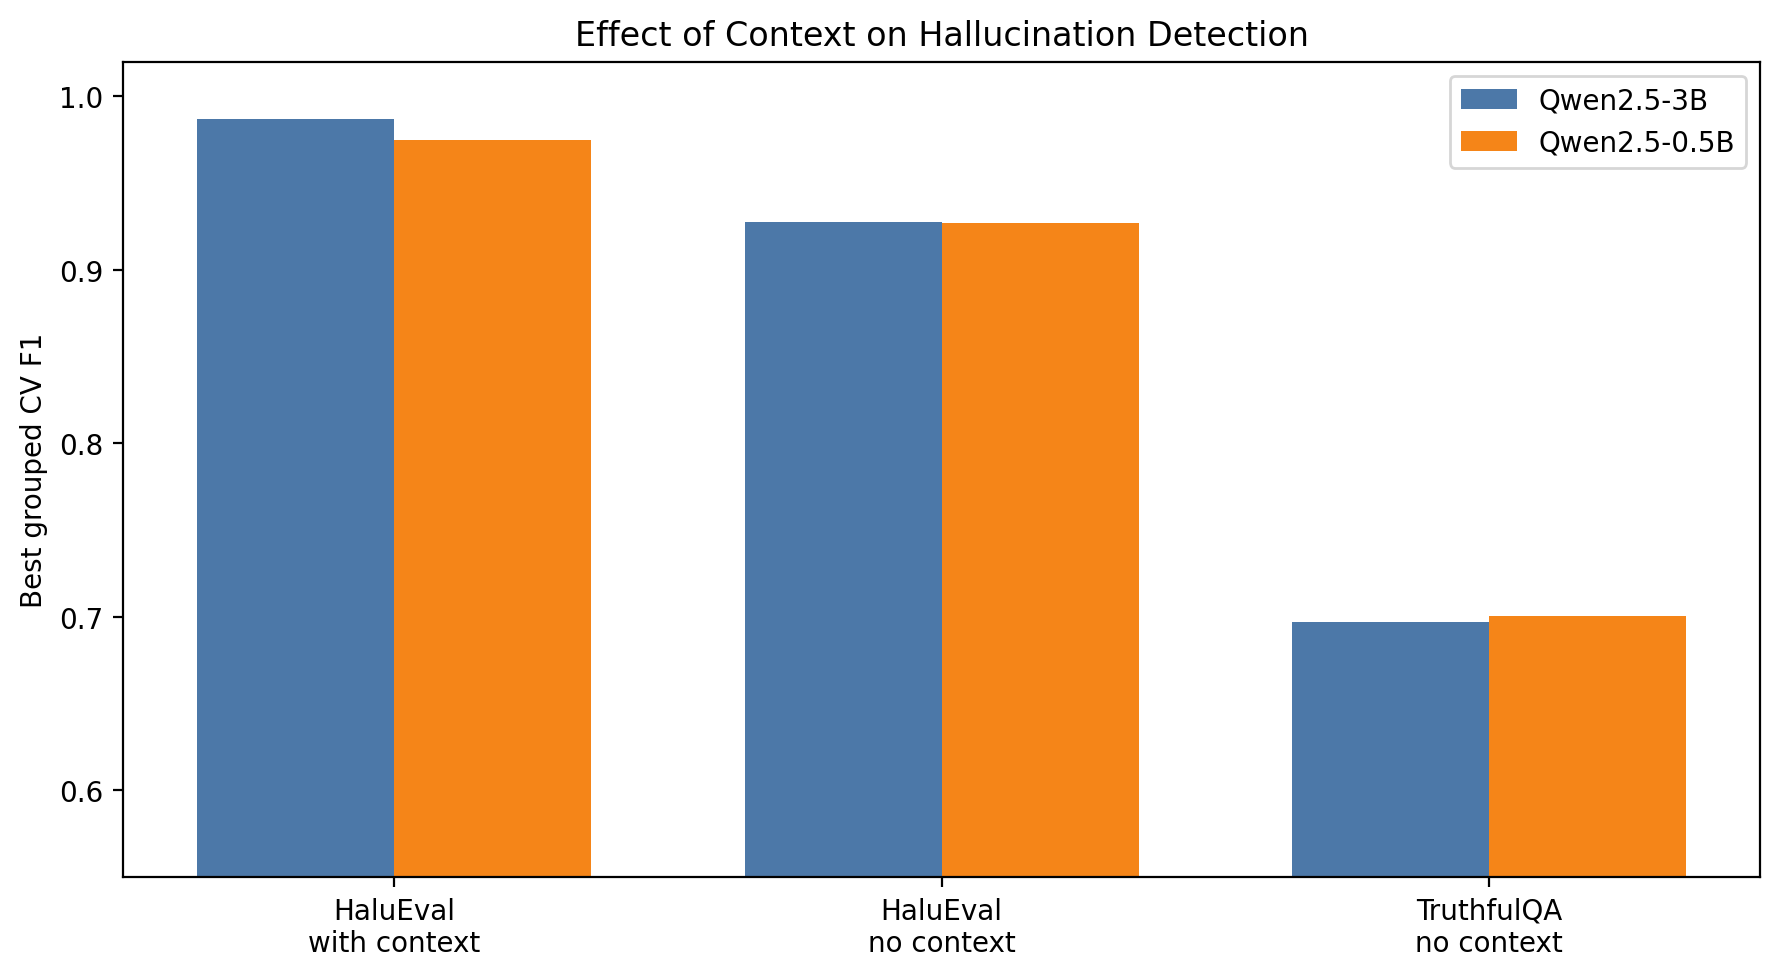
\includegraphics[width=0.85\textwidth]{../../outputs/figures/context_effect_comparison.png}
    \caption{Effect of context on grouped cross-validation F1 scores. HaluEval with context performs best, HaluEval without context drops but remains strong, and TruthfulQA remains the hardest no-context setting.}
    \label{fig:context-effect}
\end{figure}

\subsection{ROC Curves}

\begin{figure}[H]
    \centering
    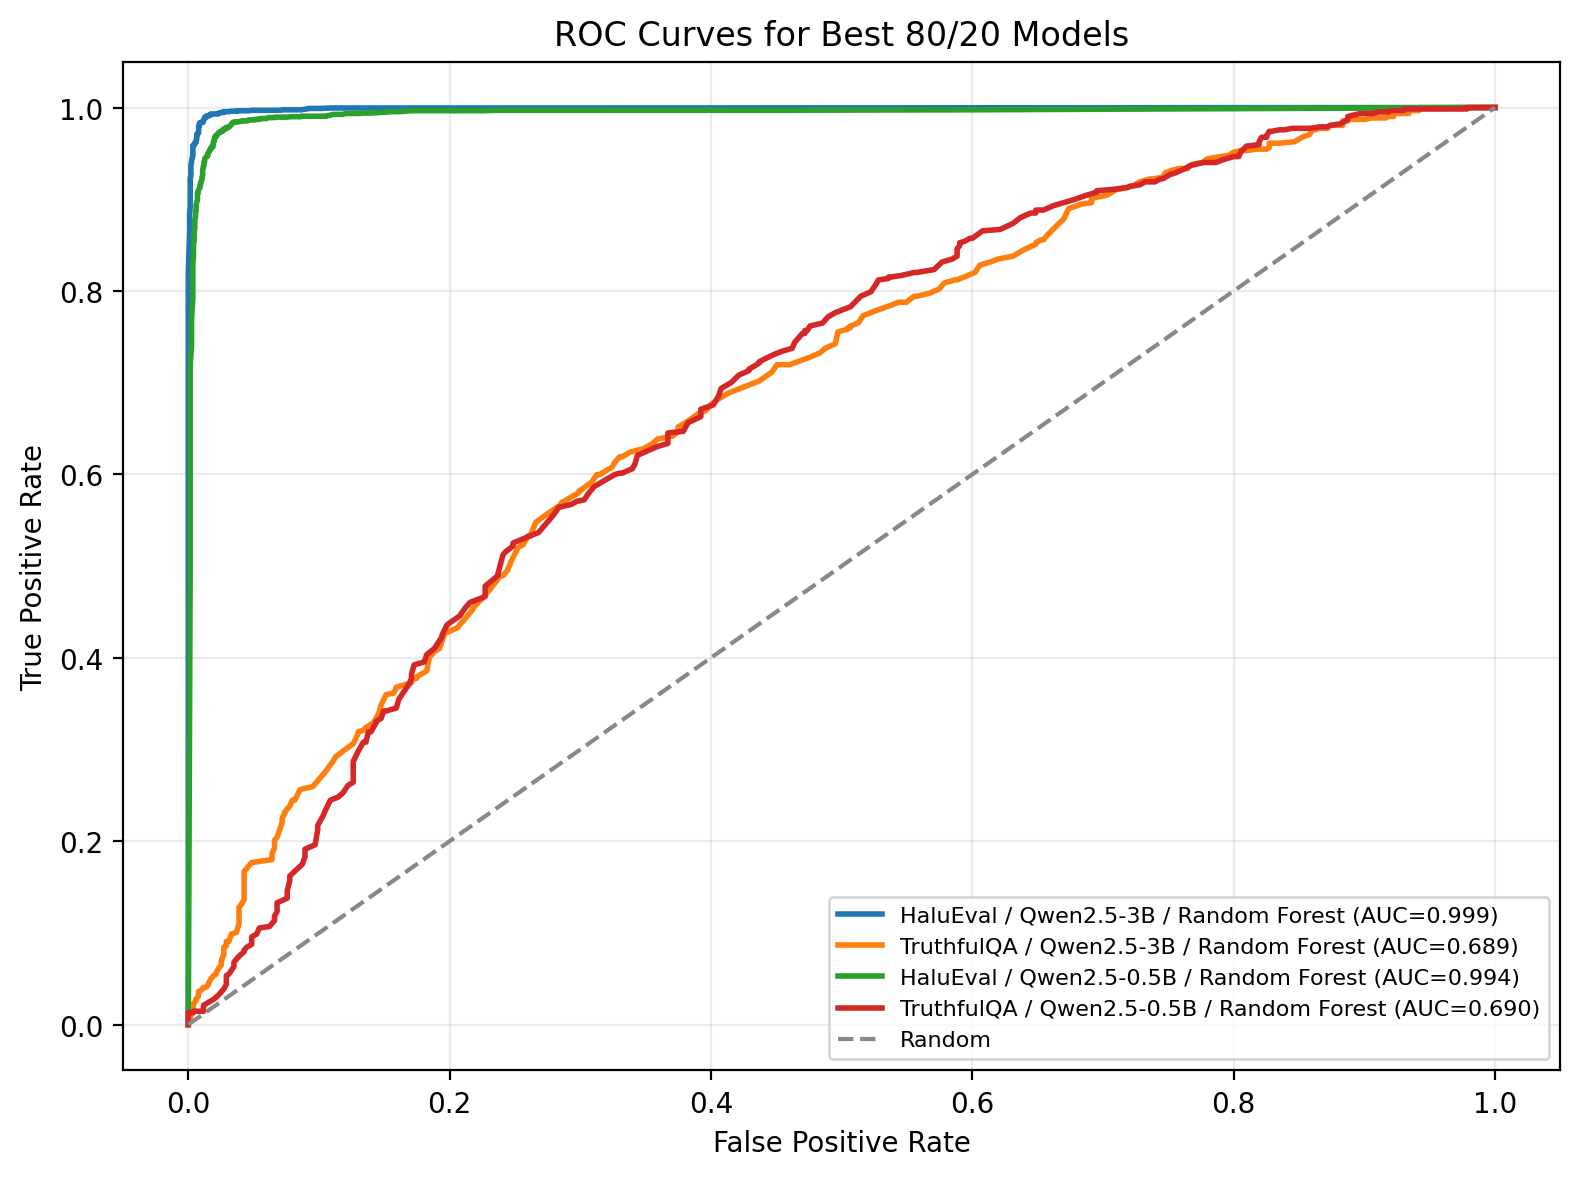
\includegraphics[width=0.85\textwidth]{../../outputs/figures/roc_curves.png}
    \caption{ROC curves for the best grouped 80/20 models.}
    \label{fig:roc-curves}
\end{figure}

\section{Ablation Study}
% TODO: Compare confidence/logprob features, entropy features, and all features.

\begin{figure}[H]
    \centering
    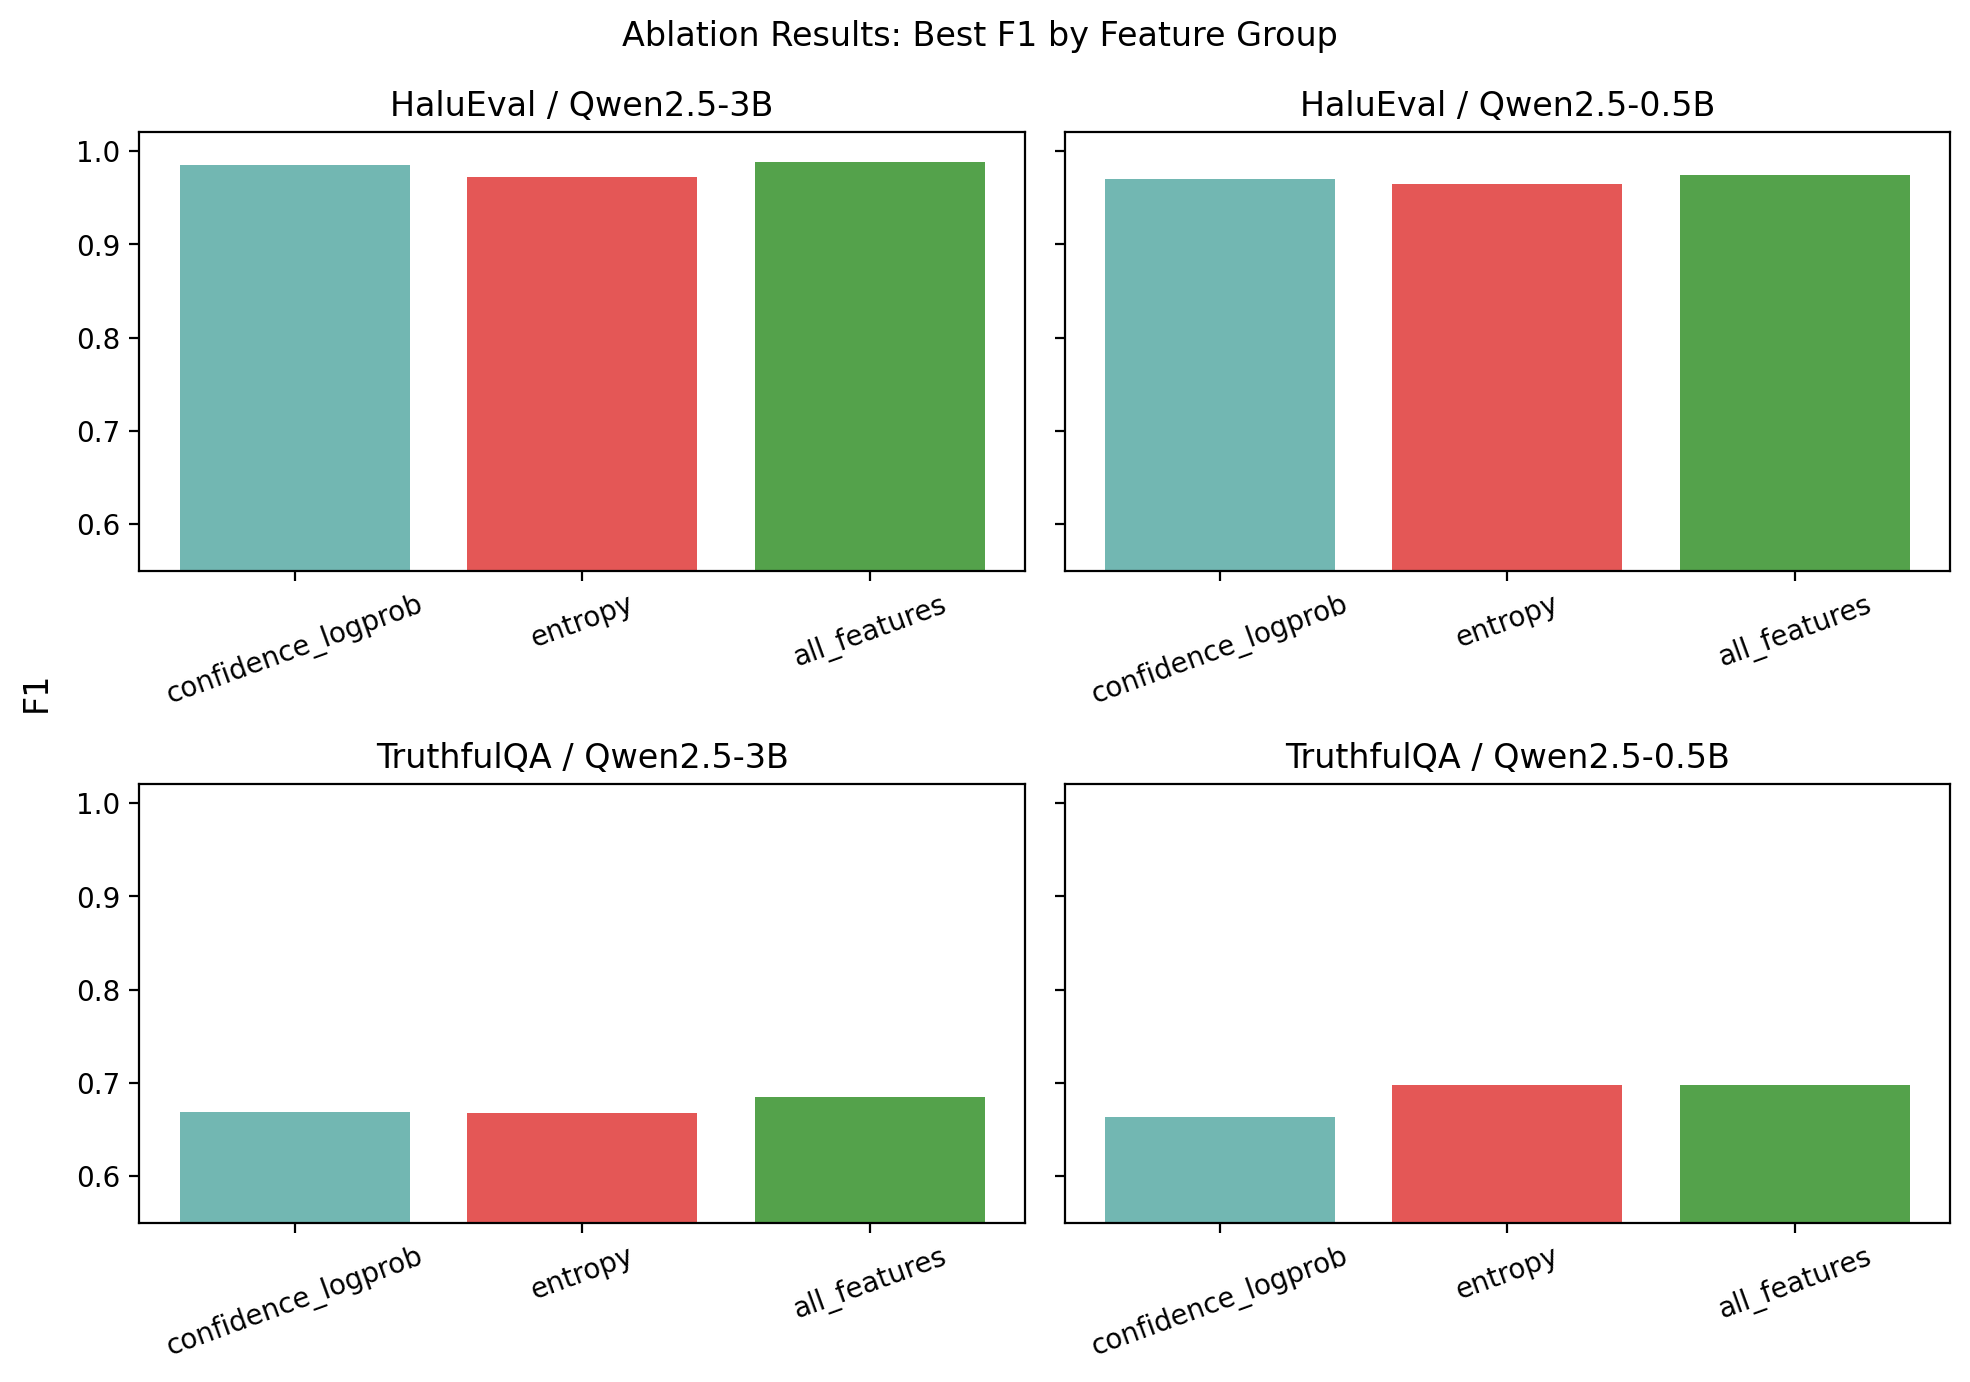
\includegraphics[width=0.85\textwidth]{../../outputs/figures/ablation_feature_group_comparison.png}
    \caption{Ablation comparison across confidence/log-probability, entropy, and all feature groups.}
    \label{fig:ablation}
\end{figure}

\section{Error Analysis}
% TODO: Explain confusion matrices and feature distribution shift.

\begin{figure}[H]
    \centering
    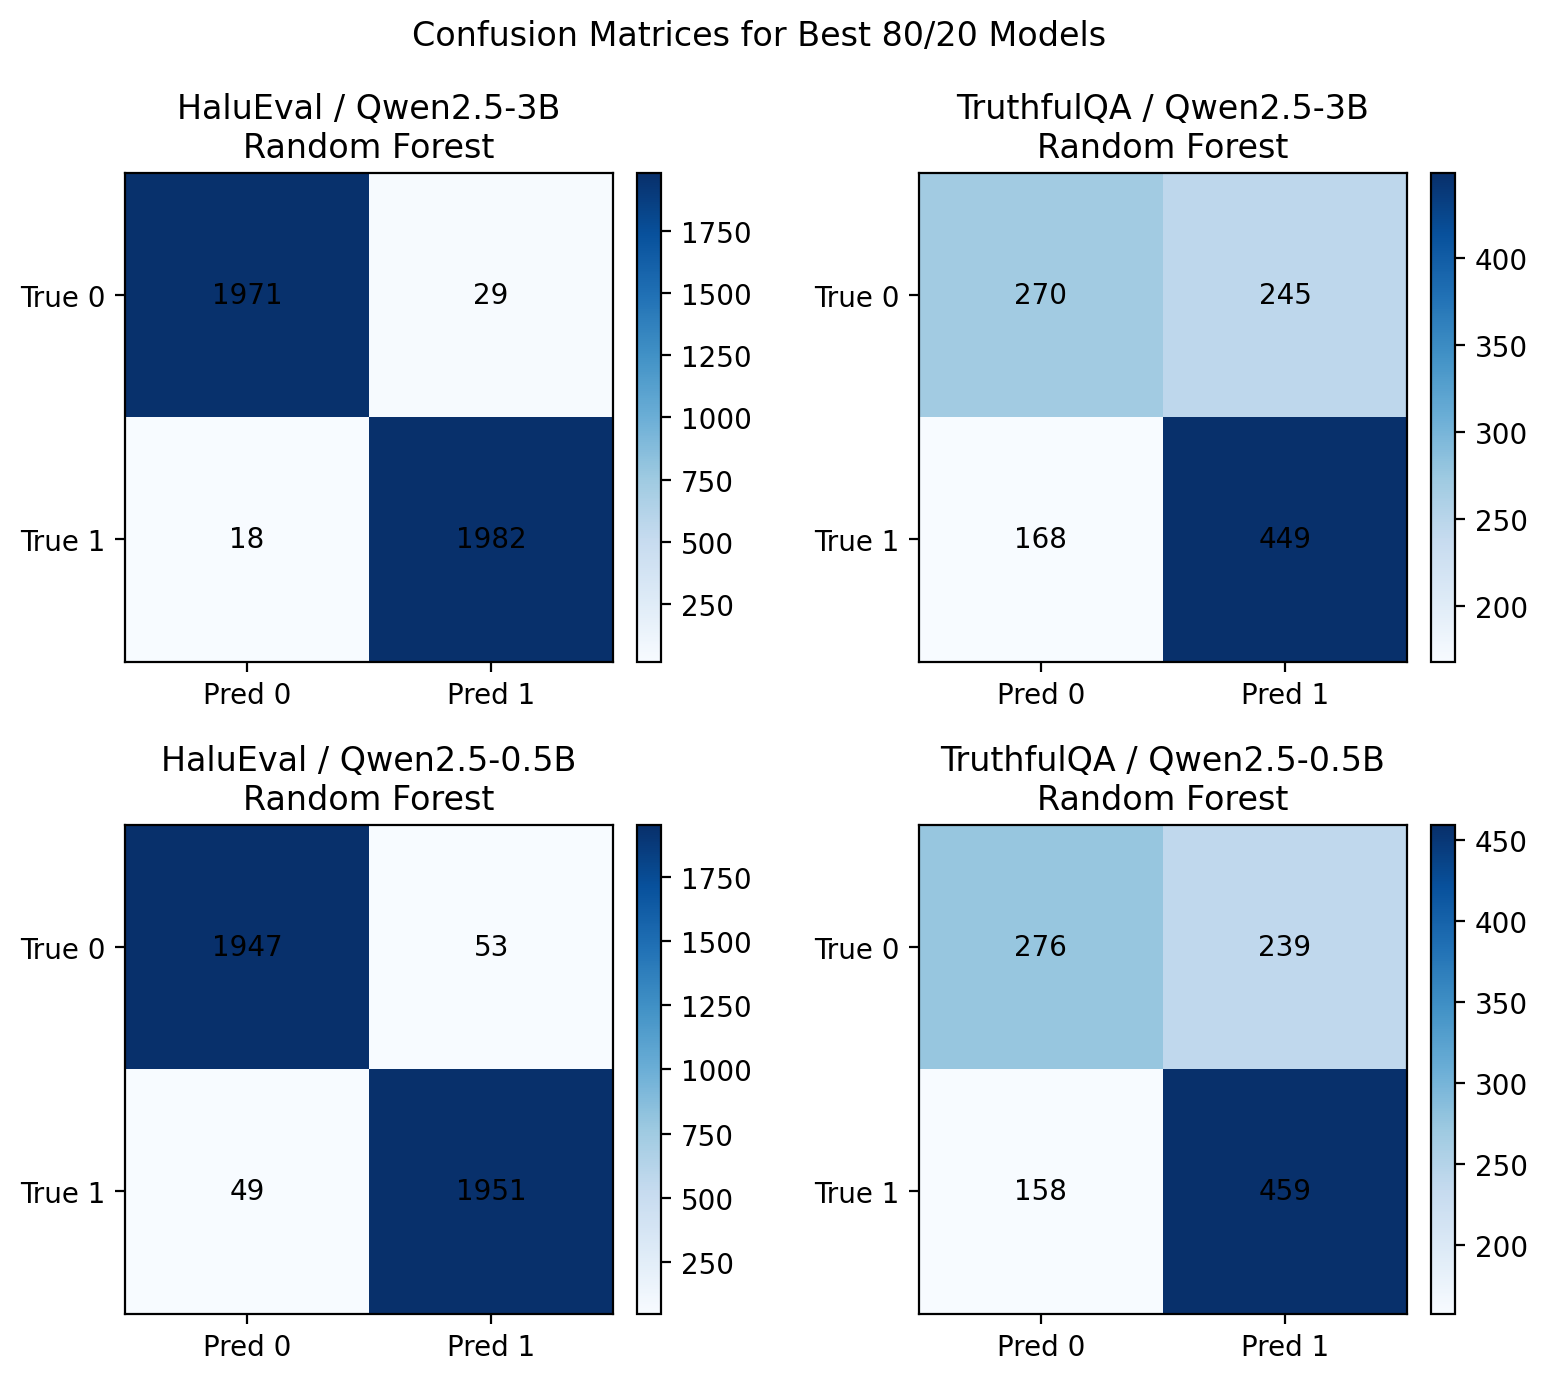
\includegraphics[width=0.85\textwidth]{../../outputs/figures/confusion_matrices.png}
    \caption{Confusion matrices for the best grouped 80/20 classifiers.}
    \label{fig:confusion}
\end{figure}

\begin{figure}[H]
    \centering
    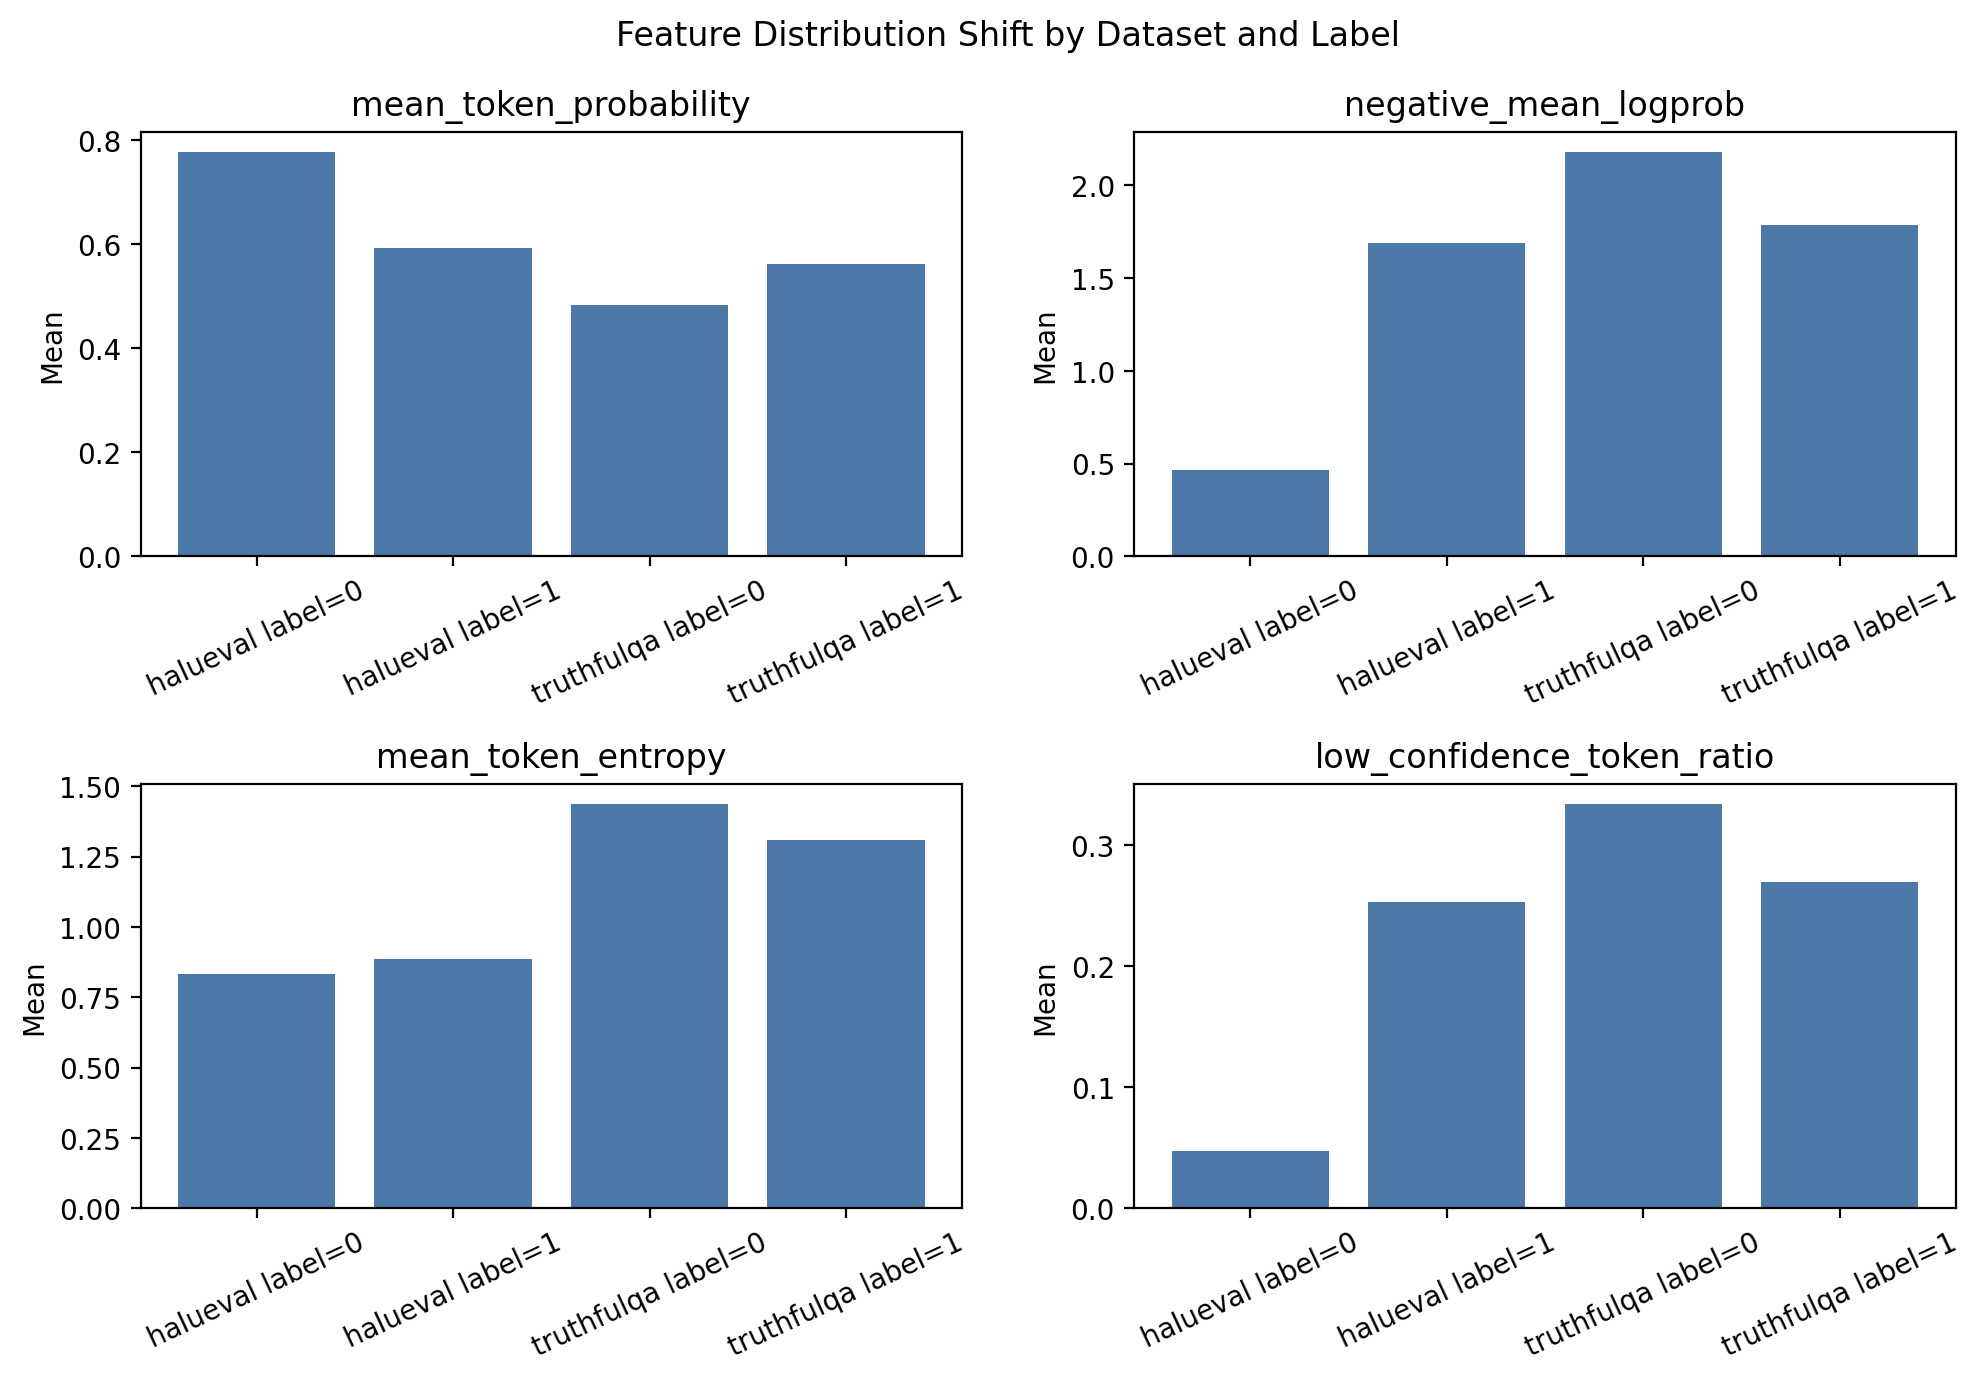
\includegraphics[width=0.85\textwidth]{../../outputs/figures/feature_distribution_shift.png}
    \caption{Selected uncertainty feature means by dataset and label.}
    \label{fig:feature-shift}
\end{figure}

\section{Discussion and Limitations}
% TODO: Discuss strong HaluEval performance, the measured effect of removing context, weaker TruthfulQA performance, dataset shift, and context dependence.

\section{Conclusion}
% TODO: Summarize the final findings and future work.

\bibliographystyle{plain}
\bibliography{references}

\end{document}
